\documentclass[12pt]{article}

\usepackage{enumitem}
\usepackage{amsmath}
\usepackage{graphicx}
\usepackage{mathtools}
\usepackage[margin=1in]{geometry}

\title{ECE 450 Notes}
\author{Anthony Jerez}

\begin{document}

    \maketitle
    \setlength{\parindent}{0pt}

    \section{Introduction to Probability}

    \textit{\textbf{Random Experiment}}: any well defined procedure 
    that produces an observable outcome that cannot be perfectly 
    predicted:
    
    \begin{enumerate}[label=(\alph*)]
        \item an outcome is called a sample point, it cannot be further 
        decomposed
        \item outcomes are disjoint; i.e. \textbf{mutually exclusive}
    \end{enumerate}
    
    \begin{center}
        $\Omega =$ Sample Space\\
        \textit{Event}: subset of the sample space
    \end{center}
    Given the set: $\Omega = \{X_1, X_2, ... , X_n\}$, there are a 
    total of $ 2^n $ possible outcomes

    \subsection{Operation on Sets}

    \begin{enumerate}
        \item Union: $A \cup B$
        \item Intersection: $A \cap B$
        \item Compliment: $A^C$
    \end{enumerate}

    \begin{enumerate}[label=(\alph*)]
        \item Two events are said to be mutually exclusive if 
        $ A \cap B = \emptyset $ can be extended to N events
        \item Events $A_1, A_2, ... , A_n$ are said to be mutually 
        exclusive (span the entire sample space) if 
        $ A_i \cap A_j = \emptyset $ for all $ i \neq j $
    \end{enumerate}

    \subsection{The 3 Axioms of Probability}

    \begin{enumerate}[label=\Roman*]
        \item $P(A) > 0$
        \item $P(\Omega) = 1$
        \item If two events are mutually exclusive, then
        $ P(A+B) = P(A) + P(B) $
    \end{enumerate}

    \begin{align}
        P\left(\bigcup_{i=1}^{n} A_i\right) = \sum_{i=1}^{n} P(A_i)\\
        P(A^C) = 1 - P(A)
    \end{align}

    \subsection{Subsets}

    $A \subset B:$ A is a subset of B, $P(A) \leq P(B)$
    \begin{align}
        P(A+B) &= P(A) + P(B) - P(AB)\\
        P(A+B+C) &= P(A) + P(B) + P(C) - P(AB) - P(AC) - P(BC) 
        + P(ABC)
    \end{align} 

    \section{Conditional Probability}

    $P(A|B):$ read as "A given B" (can be independent, i.e. no 
    relationship)
    \begin{align}
        P(A|B) = \frac{P(AB)}{P(B)}\\
        P(B|A) = \frac{P(AB)}{P(A)}
    \end{align}

    If A and B are \textit{independent}, then
    \begin{align}
        P(AB) = P(A) \cdot P(B)
    \end{align}
    \textbf{\textit{Bayes Rule}}
    \begin{align}
        P(A|B)P(B) = P(B|A)P(A)
    \end{align}

    \section{Total Probability}

    Suppose events $A_1, A_2,\dots,A_n$ are mutually exclusive and 
    exhaustive
    
    \begin{center}
        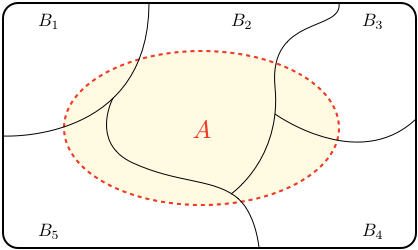
\includegraphics[scale=0.5]{images/total_prob.png}
    \end{center}
    \begin{align*}
        P(B) &= P(A_1B) + P(A_2B) + ... + P(A_nB)\\
             &= P(B|A_1)P(A_1) + P(B|A_2)P(A_2) + ... P(B|A_n)P(A_n)\\
             &= P(B) =  \sum_{i=1}^{n} P(B|A_i)P(A_i)
    \end{align*}

    \section{Combinatorics}

    Deals with counting, sampling, ordering, selection,\dots

    \subsection{Basic Concept of Counting}

    Combined number of outcomes: $m \times n \times k$\dots

    \textbf{Example:} How many passwords can you create such that 
    the first two are small letters, next one is a capital letter, 
    and the last four are numbers?
    $$26\times 26\times 26\times 10\times 10\times 10\times 10 = n$$

    \textbf{Example:} Given a hacker generates $10^8$ passwords (can 
    be repeated) what is the probability that at least one password 
    will match yours?
    \begin{align*}
        P(passwordMatches) &= \frac{1}{N}\\
        P(passwordDoesNotMatch) &= 1 - \frac{1}{N}\\
        P(allPasswordsDoNotMatch) &= \left(1-\frac{1}{N}\right)^{10^8}\\
        P(atLeastOneMatch) &= 1 - \left(1-\frac{1}{N}\right)^{10^8}
    \end{align*}

    \subsection{Permutations}

    \textit{\textbf{Example:}} Suppose we have n distinguishable 
    objects. How many ways can you arrange the objects? 
    \textit{(without replacement)} 
    $$n!$$
    \textit{with replacement}
    $$n^n$$

    Now suppose we are interested in choosing k objects out of n 
    $(k \leq n)$, \textit{without replacement}; order is 
    \textit{important}
    $$n(n-1)(n-2)...(n-k+1)$$
    \begin{align}
        =\frac{n!}{(n-k)!}
    \end{align}

    \textit{with replacement (given k terms)}
    \begin{align}
        n(n)(n)...(n) = n^k
    \end{align}

    \textbf{Example:} You have a bookshelf with 4 math books, 3 
    physics, 2 economics, and 1 history book. How many ways can you 
    arrange the bookshelf such that similar books are bundled/adjancent?

    Ways of arranging the books:
    $$(4!)(3!)(2!)(1!)$$
    Now account for the ways you can arrange the bundles:
    $$(4!)(3!)(2!)(1!)(4!)$$

    \textbf{Example:} Ways of creating a password of 5 numbers 
    without replacement:
    $$\frac{10!}{(10-5)!}$$

    \textit{\textbf{Combination:}} How many ways can you select k 
    objects out of n distinguishable objects without replacement 
    (n choose k); order does \textbf{not} matter
    \begin{align}
        \frac{n!}{(n-k)!k!} = \binom{n}{k}
    \end{align}

    *note that $\binom{n}{n-k}$ is the same thing\\[\baselineskip]
    \textbf{Example:} Given a deck of cards, you choose 5 cards. 
    What is the probability you get two aces?
    $$\frac{\binom{4}{2}\binom{48}{3}}{\binom{52}{5}}$$

    \textbf{Example:} A team has 25 players, 15 are position players, 
    10 are pitchers. The lineup consists of 9 players.
    \begin{enumerate}[label=(\alph*)]
        \item How many lineups can the manager create?\\
        $\binom{10}{1}\binom{15}{8} = \frac{(10)(15!)}{(7!)(8!)} = 64350$
        \item How many batting orders can he create?\\
        $64350(9!)$
    \end{enumerate}

    \textbf{Example:} Suppose you pick 3 cardsfrom a deck. What is 
    the probability of getting atleast an ace?
    \begin{align*}
        &= 1 - P(noAce)\\
        &= 1 - \frac{\binom{48}{3}}{\binom{52}{3}}
    \end{align*}

    \textbf{Example:} Suppose you have 2 letters, A and B. How many
    sequences can you generate having 3 As and 5 Bs. 
    \begin{align*}
        &=\binom{8}{3} \times \binom{5}{5}\\
    \end{align*}

    \textbf{Example:} You have 4 mailboxes and 8 indistinguishable 
    balls. (a) How many ways can you distribute the balls so that no 
    box is empty. Let $x_1$ be the number of balls in box 1. We know 
    $x_1+x_2+x_3+x_4 = 8$. $x_i$ is $>$ 0 for all $i$. 
    $$- - - - - - - -$$

    Since there are 7 spaces, we choose three to split them up 
    in any box.
    $$\binom{n-1}{k-1}$$
    (b) How many ways can you distribute the balls into the boxes? 
    A box can be empty.
    \begin{center}
        let $y_i = x_i + 1$ so \\
        $y_1+y_2+y_3+y_4 = 12$\\
        $$\binom{11}{3}$$
    \end{center}

    $$\sum_{k=0}^{n}\binom{n}{k} = \binom{n}{0} + \binom{n}{1} + ...
     + \binom{n}{n} = 2^n$$

    \subsection{Multinomial Coefficients}

    Suppose we have n distinguishable objects. We want to break them 
    into k groups. $G_1$ has $n_1$ objects, $G_2$ has $n_2$ objects,
    $G_k$ has $n_k$ objects. $n_1 + n_2 + ... + n_k = n$. How many ways
    can we do it?
    $$\binom{n}{n_1}\binom{n-n_1}{n_2}\binom{n-n_1-n_2}{n_3}...
    \binom{n_1-...-n_{k-1}}{n_k}$$
    \begin{align*}
        = \frac{n!}{n_1!n_2!...n_k!}
    \end{align*}

    \section{Random Variables}

    A random variable (X) is a function mapping the outcomes of a 
    random experiment into the real line. Mapping must be 1 to 1 
    \textit{or} many to 1.Mapping 1 to many is \textit{unacceptable}.

    \textbf{Example:} Suppose you toss a coin twice. 
    $$\Omega = {HH, HT, TH, TT}$$
    X is a random variable as the number of heads. X can take the 
    value 0, 1, 2
    $$P(X=0) = \frac{1}{4}$$

    \subsection{Classification of Random Variables}

    \begin{enumerate}[label = (\alph*)]
        \item \textit{\textbf{Discrete}} - said to be discrete if it 
        can take a finite or infinitely countable (i.e. integer values) 
        number of values
        \item \textit{\textbf{Continuous}} - continuous if it can take 
        infinitely uncountable number of values (i.e. real numbers) 
        number of values
        \item \textit{\textbf{Mixed}}
    \end{enumerate}

    \subsection{How do we describe a discrete RV}

    \textit{\textbf{PMF}} - probability mass function $P(X=k)$ for 
    all possible values of k 
    $$\sum_{k}^{max}P(X=K) = 1$$

    \textit{\textbf{CDF}} - Cumulative Distributive Function
    $$F_X(x) = P(X \leq x)$$

    \begin{enumerate}[label = \Roman*]
        \item Cannot be negative
        \item Cannot slope downwards
        \item Must be a stair function and the number of stairs equals
        the number of values the random variable takes on
    \end{enumerate}

    \textbf{Example}: Suppose you toss a coin twice
    $\Omega = {HH, HT, TH, TT}$. Let $X =$ number of heads. 
    
    HH = 2, HT = 1, TH = 1, TT = 0. X is a disccrete RV taking on values 
    of 0, 1, 2. Sketch the PMF and CDF.

    PDF:
    \begin{center}
        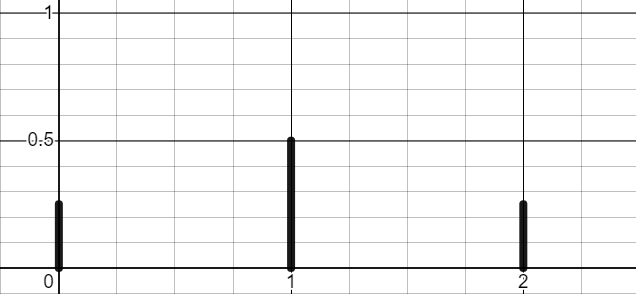
\includegraphics[scale = 0.45]{images/prob_df.png}
    \end{center}

    CDF:
    \begin{center}
        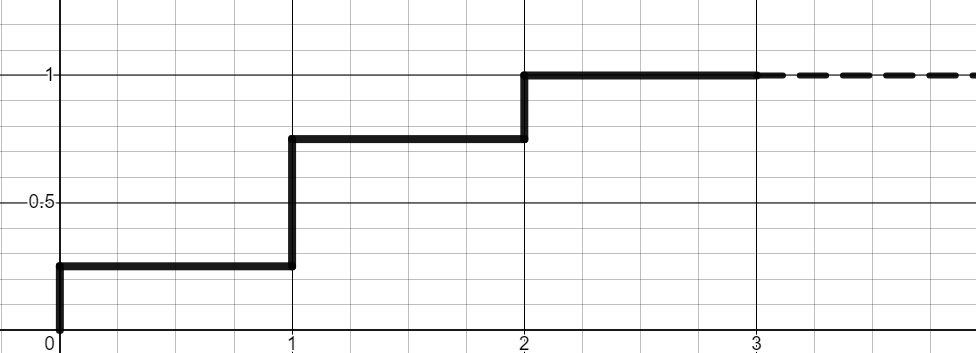
\includegraphics[scale = 0.35]{images/cdf.png}
    \end{center}
    $$F_X(1) = 3/4$$
    $$F_X(0.5) = 1/4$$
    $$P(X=0.5) = 0$$

    *Note that $<$ is denoted by a '\textit{parenthises}' on a 
    number line and $\leq$ is denoted by '\textit{brackets}'

    \textbf{Example Cases:}
    \begin{enumerate}
        \item $P(x_1 < x \leq x_2) = F_X(x_2)-F_X(x_1)$
        \item $P(x_1 \leq x \leq x_2) = F_X(x_2)-F_X(x_1)+P(X=x_1)$
        \item $P(x_1 \leq x < x_2) = F_X(x_2)-F_X(x_1)+P(X=x_1) -
        P(X=x_2)$
        \item $P(x_1 < x < x_2) = F_X(x_2)-F_X(x_1)-P(X=x_2)$
    \end{enumerate}

    \subsection{Famous Discrete Random Variables}

    \begin{enumerate}[label = \Roman*]
        \item \textit{\textbf{Bernoulli}} -\\
        Can take 1 of 2 possible values
        \item \textit{\textbf{Binomial}} - \\
        Suppose we have a bernoulli experiment repeated n times (n is
        not random). Let $X=$ number of successes in n trials
        \begin{center}
            $PMF = P(X=k)$ where $k=0,1,\dots,n$
        \end{center}
        \textbf{Example}: Suppose we toss a fair coin 3 times, let X be 
        the number of heads. Find the PMF of X 
        \begin{center}
            X is a discrete random variable that can take the values: 0, 1,
            2, \& 3
            $P(X=3) = P(HHH) = 1/8$
        \end{center}
        \begin{align}
            P(X=k) = \binom{n}{k}p^k(1-p)^{n-k}
        \end{align}
        $k=0,1,\dots,n$

        \textit{where} 
        p = probability of success in a single trial\\
        k = number of successes in n trials
        \item \textit{\textbf{Geometric}} -\\
        Number of trials until the first success; will be represented
        as a non-increasing PDF
        \begin{align}
            P(X=k) = (1-p)^{k-1}p
        \end{align}
        where $k=0,1,\dots$
        \item \textit{\textbf{Pascal}} -\\
        The number of trials until getting m successes
        \begin{align*}
            P(X=k) = \binom{k-1}{m-1}p^{m-1}(1-p)^{k-1-(m-1)} 
        \end{align*}
        \begin{align}
            \binom{k-1}{m-1}p^m(1-p)^{k-m} 
        \end{align}
        where $k = m, m+1, m+2, \dots$
        \item \textit{\textbf{Poisson}} -\\
        X is said to be a poisson with parameter $\lambda$ (average)
        \begin{align}
            P(X=k) = \frac{e^{-\lambda}(\lambda^k)}{k!}
        \end{align}
        where $\lambda = np$
        \item \textit{\textbf{Hyper-Geometric}}
        \textbf{Example}: Given a bowl, we have M red balls and N blue 
        balls. Pick L balls without replacement\\
        Let X be the number of red balls drawn:
        \begin{align}
            P(X=k) = \frac{\binom{M}{K}\binom{N}{L-K}}{\binom{M+N}
            {L}}
        \end{align}
    \end{enumerate}
\end{document}